\section{Tensor Product Surfaces}
2D to 2D mainly used for warping
No NURBS
\greenbf{Tensor Product Surface:} 2D/3D curve: $x(u) = \sum_{i=0}^mc_iF_i(u)$ with bases $F_i$ and coefficients $c_i$. For surfaces turn coefficients into functions of a second parameter: $c_i(v) = \sum_{j=0}^v\alpha_{i,j}G_j(v)$ resulting in the tensor product surface $x(u,v) = \sum_{i=0}^mc_i(v)F_i(u) = \sum_{i=0}^m\sum_{j=0}^n\alpha_{i,j}F_i(u)G_j(v)$

\greenbf{Bezier Patches:} Given bezier curve of degree m $b^m(u) = \sum_{i=0}^mb_iB_i^m(u)$ and control points $b_i$ as bezier curves of degree n: $b_i = b_i(v) = \sum_{j=0}^nb_{i,j}B_j^n(v)$ construct point on the surface: $b_{m,n}(u,v) = \sum_{i=0}^m\sum_{j=0}^nb_{i,j}B_i^m(u)B_j^n(v)$\\
\textbf{Properties:} affine invariance, convex hull, variation diminishing, boundary curves are bezier curves.

\greenbf{2D deCasteljau:} Algorithm for computing point on surface.

\greenbf{Warping:} Function from 2D to 2D, distorting an image

\greenbf{NURBS:} Non uniform rational b-splines. $\neq$  Tensor Product Surfaces since bases not separable. Top row: different B-splines, bottom row: nurb surface with different weigths
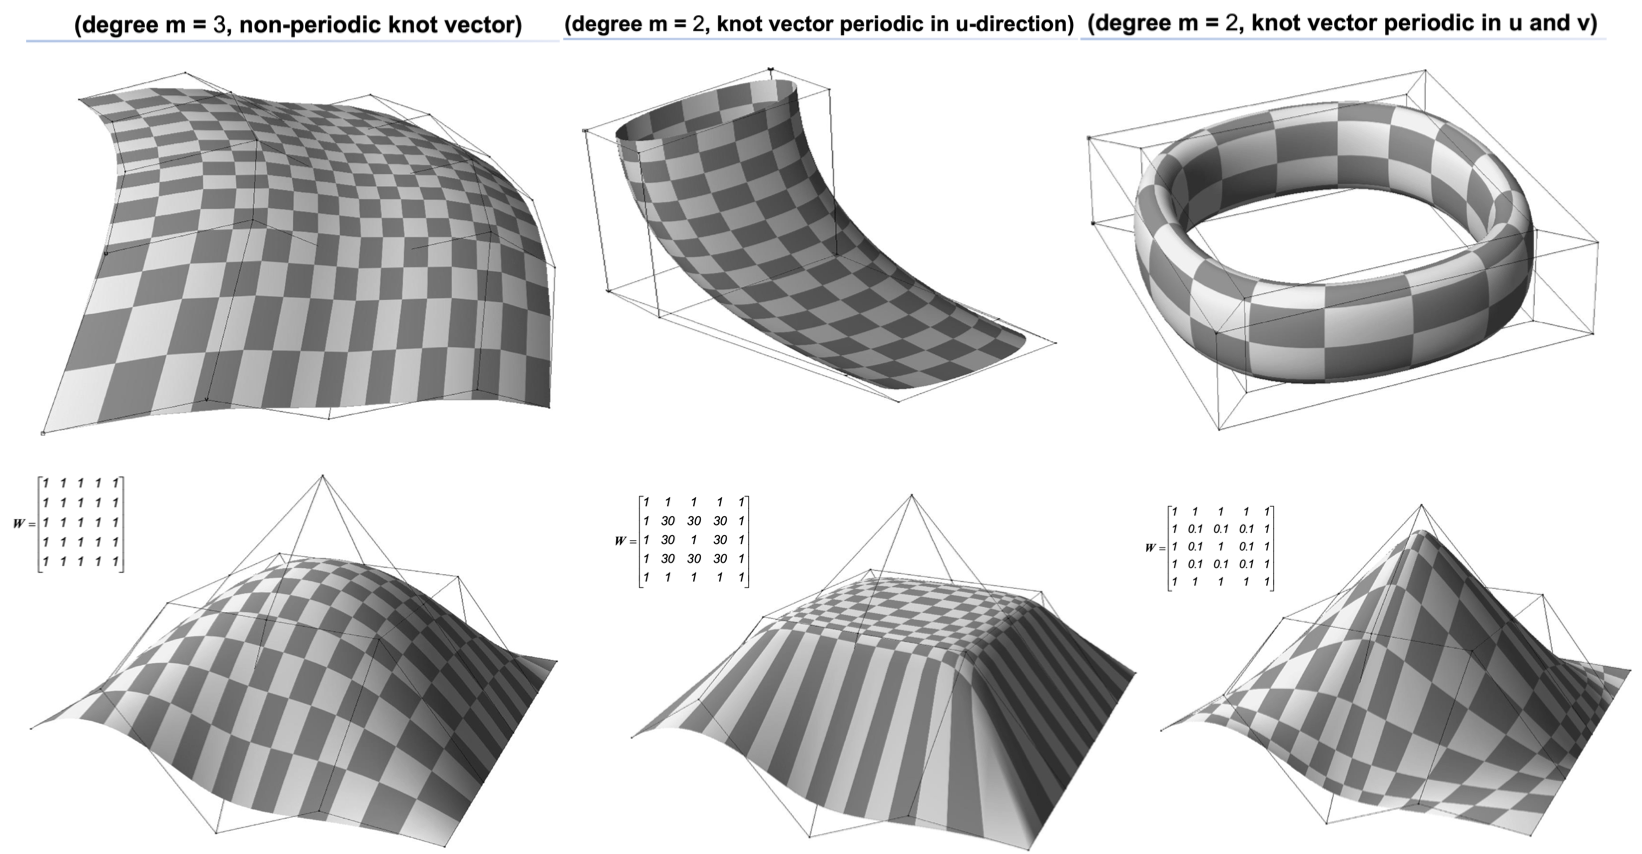
\includegraphics[width=\columnwidth]{assets/alex/bSplineSurfaces.png}